\documentclass{article}%scrartd

\usepackage{graphicx}
\usepackage{amsmath}

\begin{document}

\section{Auswirkung von Dezimation}
	Es wird ein 110Hz Rechteck aufgenommen. Die Abtastrate beträgt 15kHz. Um Allaising zu
 	vermeiden, wurde ein Antiallaisingfilter ("die blaue Box") verwendet. Anschließend wird das
	Amplitudenspektrum bestimmt und geplottet.\\

\subsection{Dezimation von gemessenen Signalen}

	\begin{figure}[htb]
		\centering
		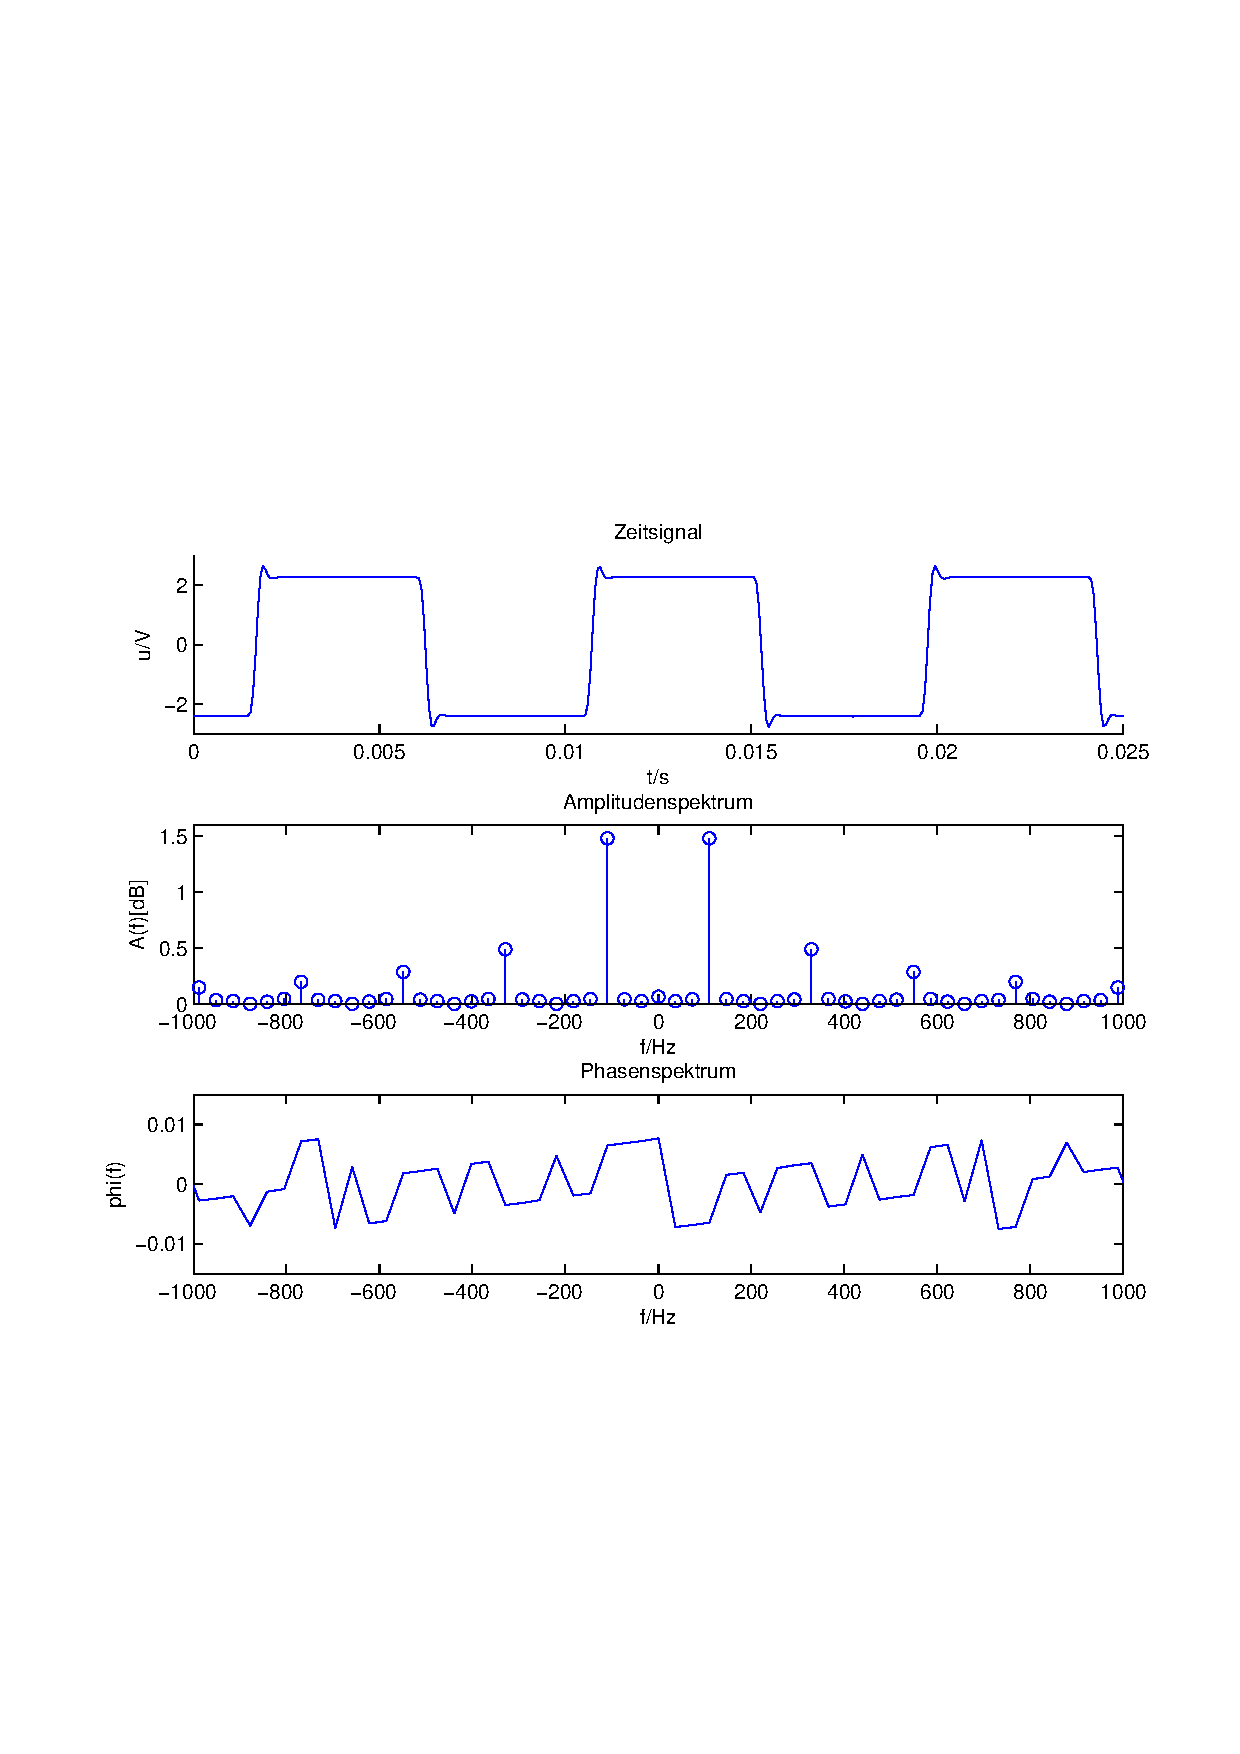
\includegraphics[width=1\textwidth]{rechteck_100Hz_15kHz_frequenzbegrenzung.pdf}
		\caption{aufgenommener Rechteck und sein Spektrum, auf 1kHz begrenzt}
	\end{figure}

	Das Spektrum sieht wie erwartet aus. Die Spektramlinien sind klar zu erkennen. Die kleineren
 	Amplituden um die Spektrallinien herrum sind minimale Oberwellen, da perfekte Rechtecke mit der
 	Messkette nicht erfasst werden können. Dennoch ist das Messsignal sehr gut angenähert.\\
	Nun wird eine Nachabtastung (Dezimation) durchgeführt. Die Nachabtastung erfolgt mit 3kHz. Dies
 	läuft effektiv darauf hinaus das ein Messwert gespeichert und die folgenden vier gelöscht werden.
 	Nach der Nachabtastung ist also nurnoch ein fünftel der Messwerte vorhanden.\\
	Auch das nachabgetastete Spektrum wird geplottet.

	\begin{figure}[htb]
		\centering
		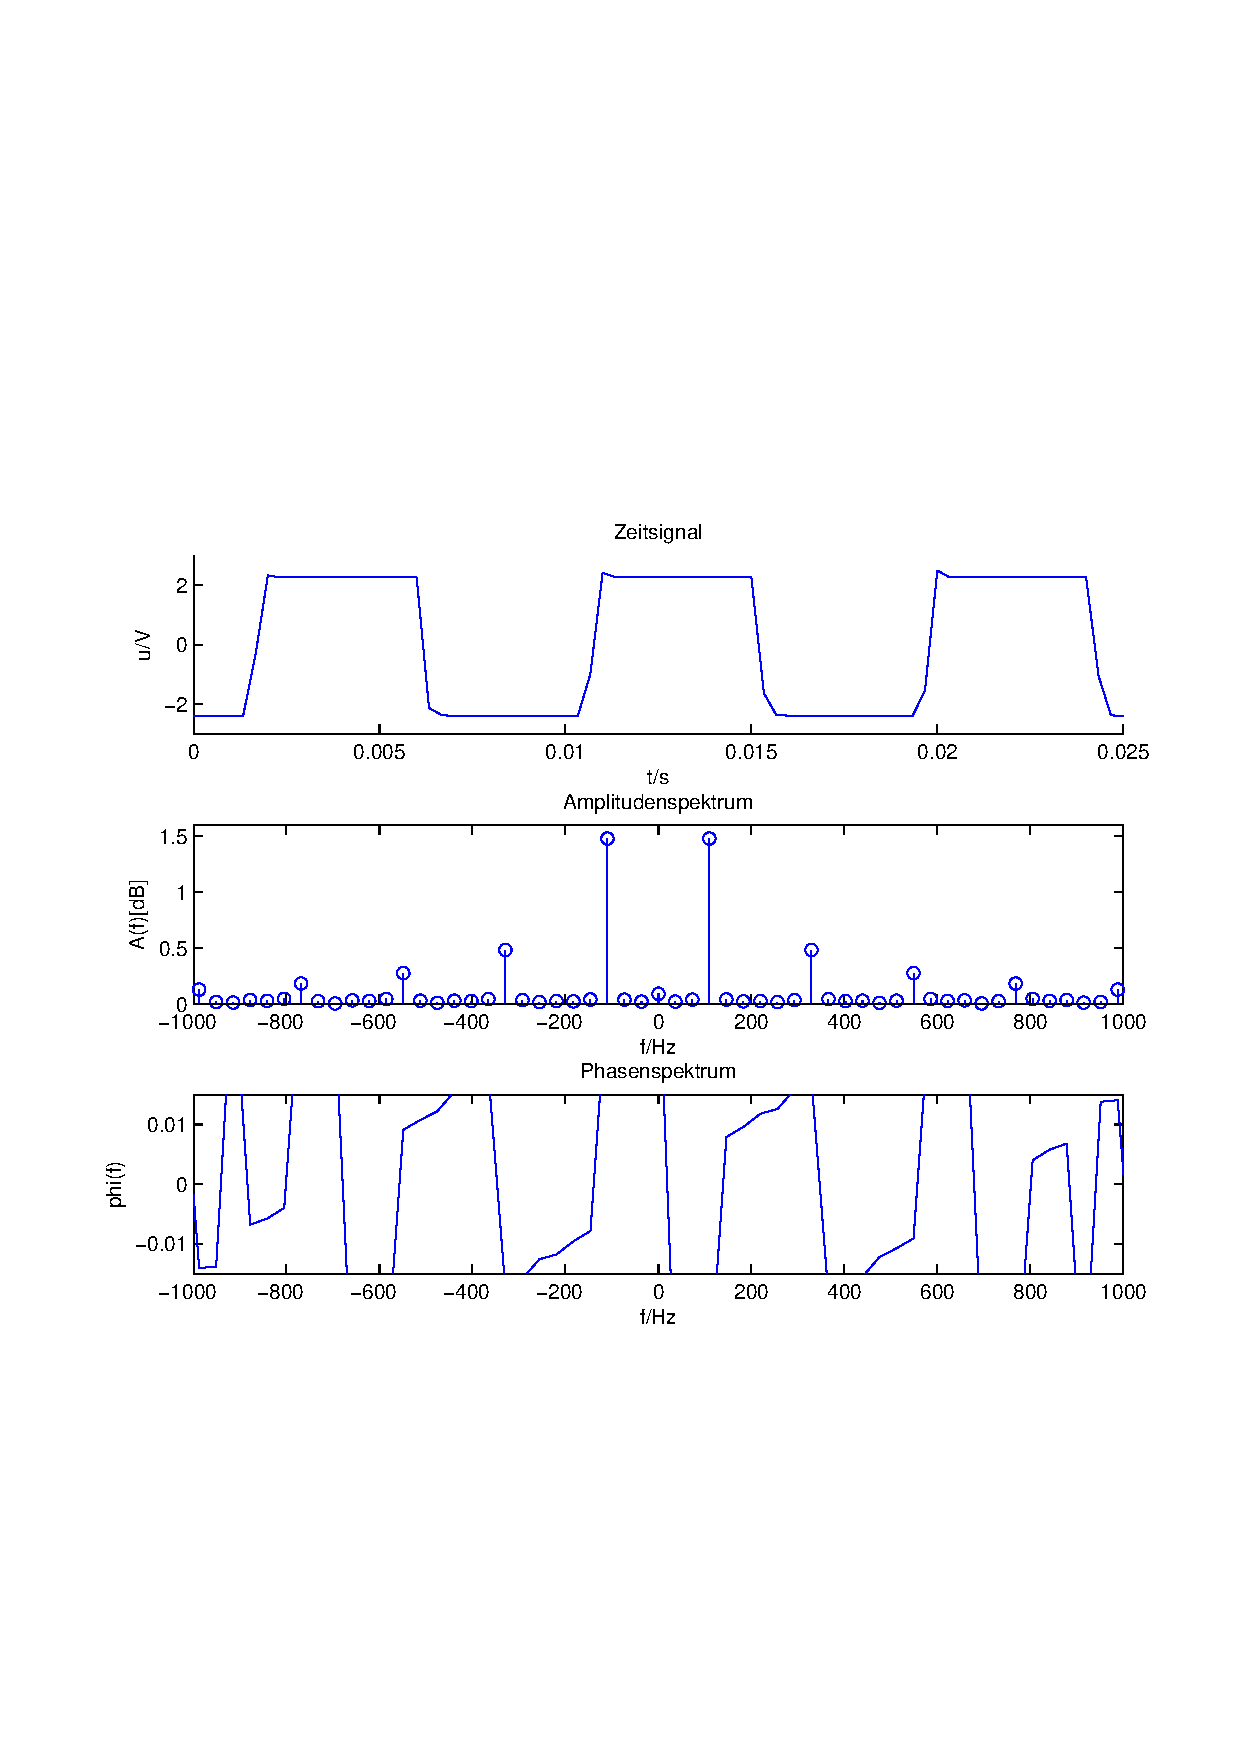
\includegraphics[width=1\textwidth]{rechteck_100Hz_15kHz_3kHz_nachabgetastet_frequenzbegrenzung.pdf}
		\caption{aufgenommener rechteck nach der Nachabtastung}
	\end{figure}	

	Bei einer diskreten Fourirtransformation erhält man für das Frequenzspektrum genau so viele
 	Stützstellen, wie das Signal Abtastpunkte hat. Daher muss das nachabgetastete Signal nur ein 	
	Fünftel der Spektrallinien haben.\\
	Auf dem Plot scheint es so, das sich die Anzahl der Spektrallinien nicht geändert hat. 

	\begin{figure}[htb]
		\centering
		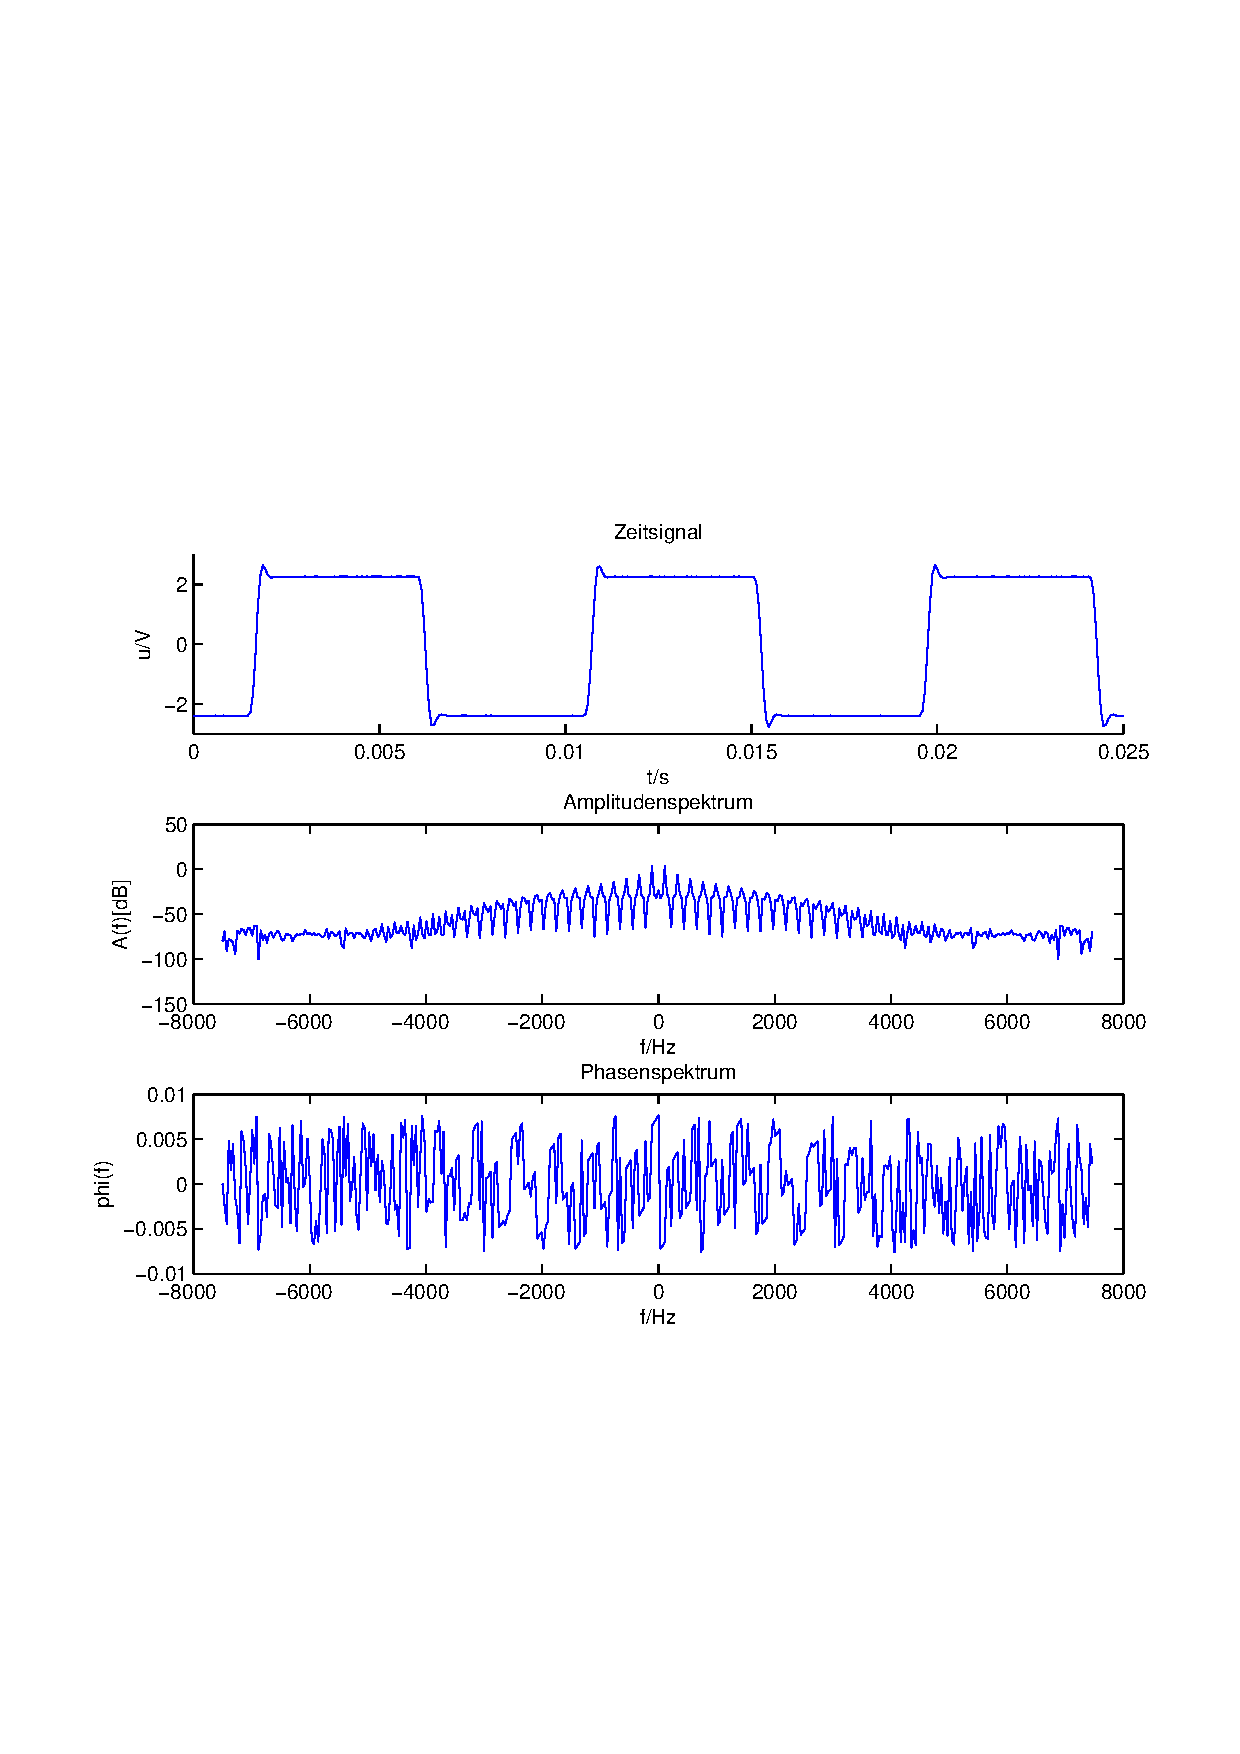
\includegraphics[width=1\textwidth]{rechteck_100Hz_15kHz_keine_frequenzbegrenzung.pdf}
		\caption{gesamtes Spektrum des afgenommenen Rechtecks}
	\end{figure}	

	\begin{figure}[htb]
		\centering
		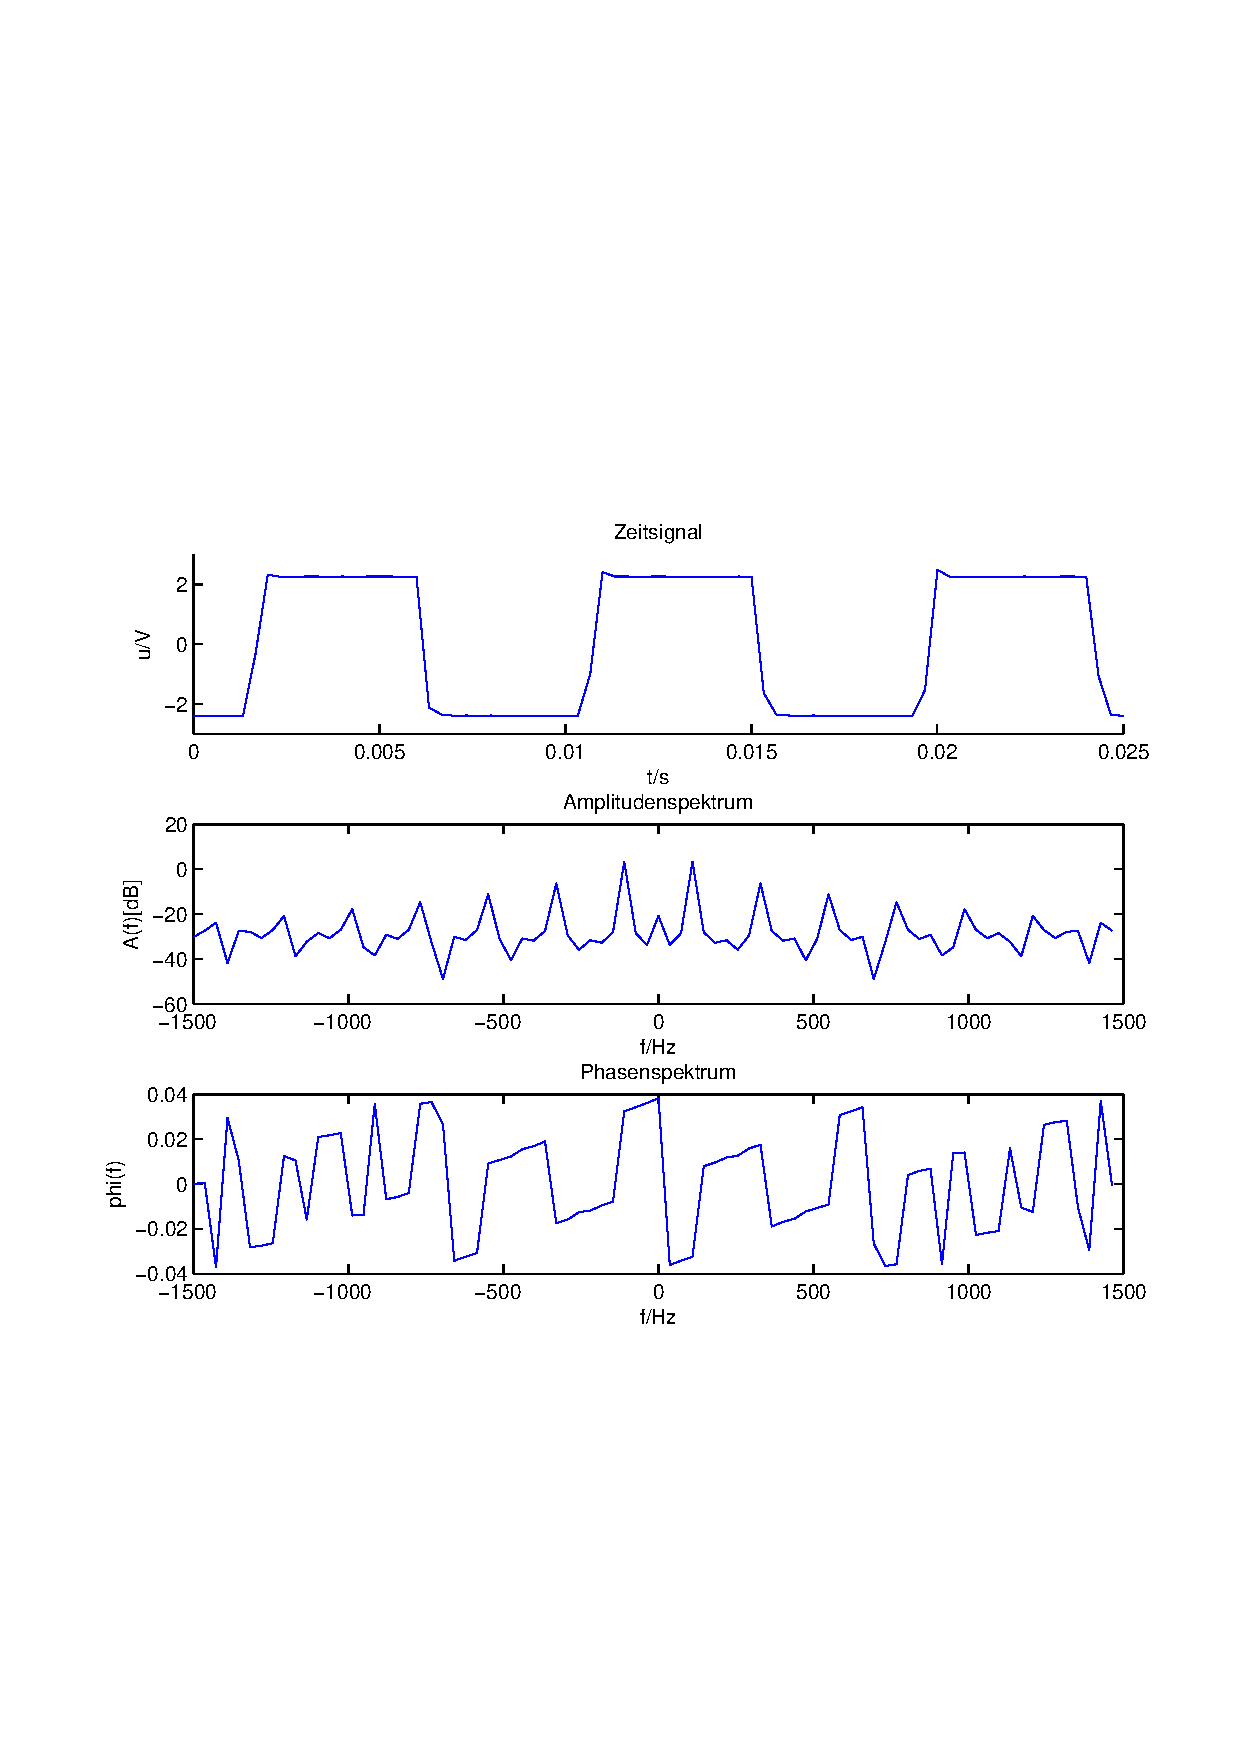
\includegraphics[width=1\textwidth]{rechteck_100Hz_15kHz_3kHz_nachabgetastet_keine_frequenzbegrenzung.pdf}
		\caption{gesamtes Spektrum des nachabgetasteten Signals}
	\end{figure}	

	Das Spektrum des Nachabgetasteten Signals hat zwischen den einzelnen Spektrallinien den gleichen Abstand wie das Spektrum des 
	unbearbeiteten Signals. Allerdings fehlen die höheren Frequenzen, da diese nun nicht mehr mit einer Abtastfrequenz erfasst werden 
	können, die geringer ist als sie selbst. Daher ist das Spektrum des nachabgetasteten Signals nun schmaler als die des ursprünglichen 
	Messsignals.\\

	Da die wichtigen Spektrallinien im Bereich bis 1kHz liegen wird nun dieser Bereich betrachtet. In der Nahansicht des Spektrums fällt auf,
 	dass der Oberwellenanteil im Spektrum gestiegen ist.\\
	Diese Frequenzanteile entstehen durch die Nachabtastung. Bei der Nachabtastung des 7,5kHz Signals, wird das Signal mit einer Frequenz 
	von 3kHz abgetastet. Dadurch kommt es zu Allaising.\\

\subsection{Verhinderung von Allaising}

	Um kein Allaising durch Nachabtastung zu verursachen, müssen vor der Nachabtastung die Frequenzanteile, die zu hoch sind, aus dem 
	gemessenen Signal entfernt werden. Dies kann durch digitale Filterung geschehen.\\

	Nun wird das mit 15kHz abgetastete Signal vor der Nachabtastung gefiltert. Die Grenzfrequenz des digitalen Filters liegt bei 1kHz. Die 
	Nachabtastung erfolgt mit 3kHz. Dadurch kann es nun nicht mehr zu Allaising kommen. 

	\begin{figure}[htb]
		\centering
		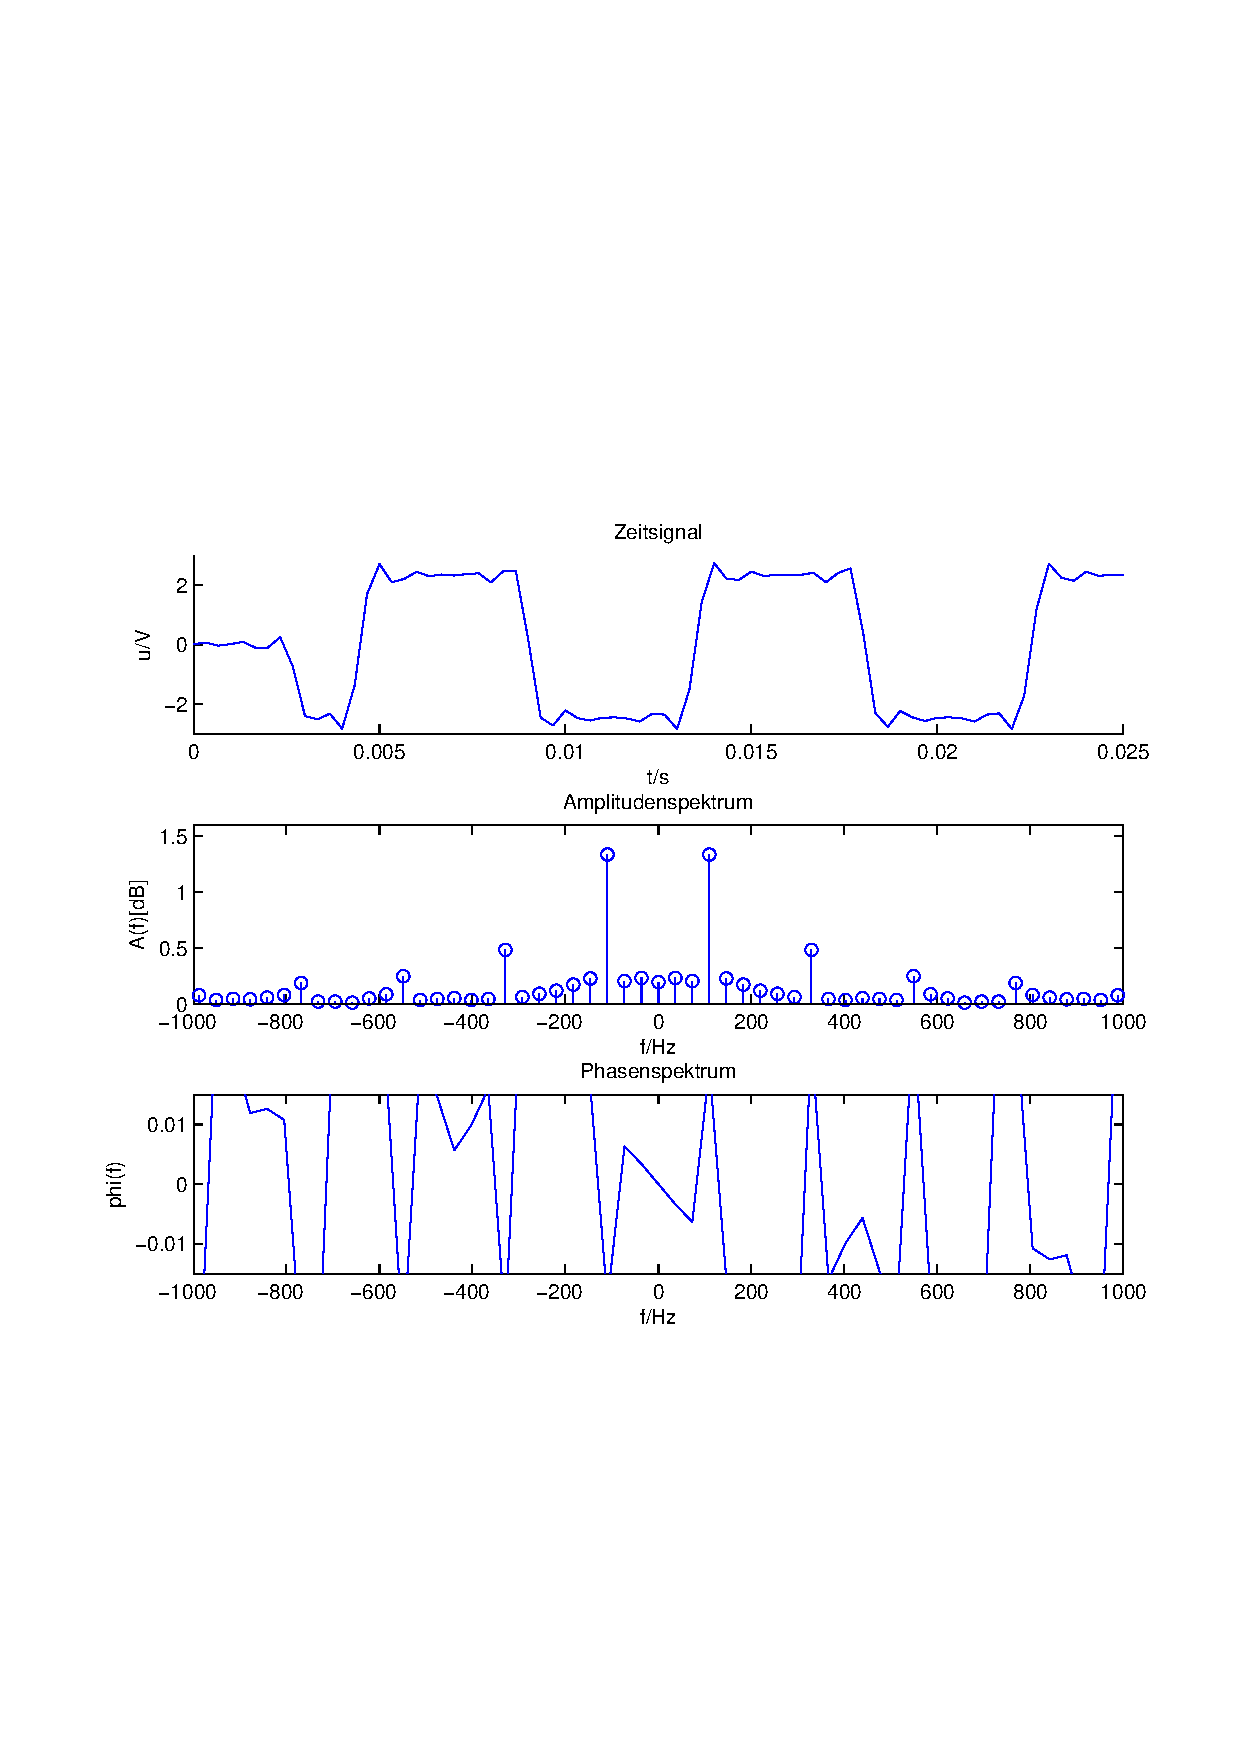
\includegraphics[width=1\textwidth]{rechteck_100Hz_gefiltert_15kHz_3kHz_nachabgetastet.pdf}
		\caption{digital gefiltertes und anschließend dezimiertes Signal}
	\end{figure}	

	Durch den Filter kann es nun nicht mehr zu Allaising kommen. Allerdings benötigt der Filter viel Zeit um sich einzuschwingen. Selbst im 
	eingeschwungenen Zustand gehen viele Details verloren. Das ist auch im Spektrum bemerkbar. Wirklich deutlich tritt nur noch die 
	Grundschwingung des Rechtecks hervor. Alle anderen Frequenzanteile werden sehr stark gedämpft. Die Messung ist nicht mehr 	
 	aussagekräftig.
	
\subsection{Optimierung der Nachabtastung}

	Die digitale Filterung ist sehr Rechenintensiv. Bei der Dezimation werden die meisten Messwerte aber sofort wieder verworfen. Filterung 
	und Dezimation lassen sich kombinieren und dadurch viel Rechenzeit sparen. In der Funktion DecimFilt() wird nur jeder 5te Messwert 
	überhaupt gefiiltert. Dadurch wird viel Rechenzeit gespart. Das Ergebnis unterscheidet sich nicht von einer digitalen Filterung mit 
	anschließender Nachabtastung. Abweichungen sind durch den unterschiedlichen Anschnitt des Rechtecks bedingt.

	\begin{figure}[htb]
		\centering
		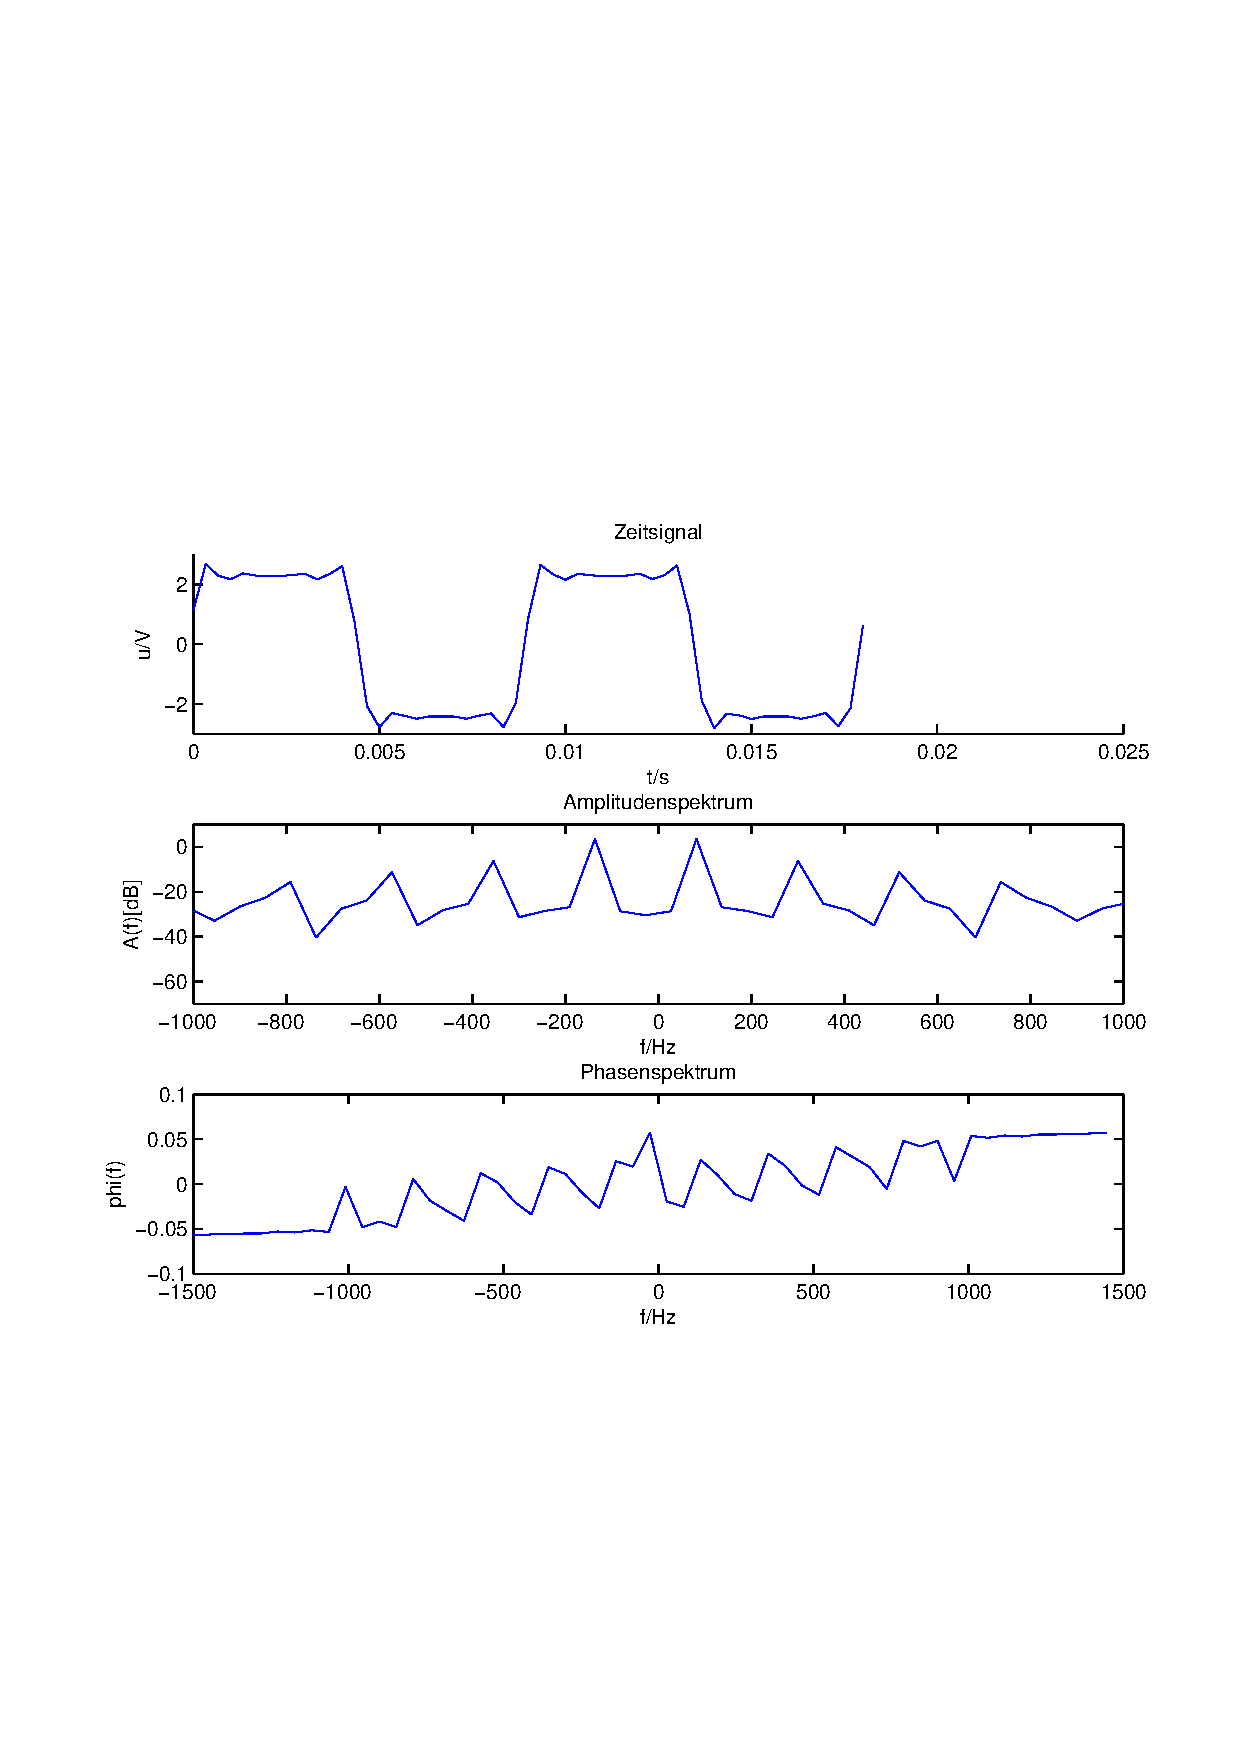
\includegraphics[width=1\textwidth]{rechteck_100Hz_decimFilt_15kHz_3kHz_nachabgetastet.pdf}
		\caption{Signal das mit DecimFilt() gefiltert und dezimiert wurde}
	\end{figure}	

\end{document}